\documentclass[a4paper,10pt]{article}

\usepackage[margin=2cm]{geometry}
\usepackage{verbatim}% http://ctan.org/pkg/verbatim
\usepackage{caption}
\usepackage{etoolbox}
\usepackage{cprotect}
\usepackage{xcolor}
\usepackage{graphicx}

\newcommand{\question}[1]{#1}
\newcommand{\solution}[1]{}
\newcommand{\lessonplan}[1]{}

\newtoggle{showsol}
\newtoggle{showlessonplan}
%only one of the below should be not commented otherwise bottom one happens
\togglefalse{showsol}\togglefalse{showlessonplan} %question sheet only
%\toggletrue{showsol}\togglefalse{showlessonplan} %solution sheet
%\togglefalse{showsol}\toggletrue{showlessonplan} %lesson plan

\iftoggle{showsol}
{
	\renewcommand{\solution}[1]{\textcolor{blue}{\\ \textbf{Solution}} \\#1}
	\renewcommand{\question}[1]{}
}
{}

\title{List of lists of references -- follow the links\solution}

\iftoggle{showlessonplan}
{
	\title{List of lists of references -- follow the links\\\textcolor{blue}{Lesson Plan}}
	\renewcommand{\lessonplan}[1]{#1}
	\renewcommand{\question}[1]{}
}{}
\date{}
\begin{document}

\maketitle



\section*{Objectives}

\noindent The \textbf{objectives of this activity} are:
\begin{itemize}
  \item To become familiar with lists of lists
  \item To become familiar with algorithms involving lists
\end{itemize}

\lessonplan{
	\fbox{\begin{minipage}{\textwidth} 
			\textbf{Time: } 30  minutes  \\
			\textbf{Aims: } To become familiar with nested loops and nested lists.\\
			\textbf{Materials:} String/thread, Scissors and bluetac (or equivalent)\\
			\textbf{Procedure:} \begin{itemize}
				\item Give each table some string (pre cut up or give scissors) and bluetac
				\item students draw up rectangles for the two lists with squares for the cells within them.
				\item students connect together the lists with their contents using string/thread
				\item students follow the links to see what changes
				\item values are written down (on paper or whiteboard) by students as each is computed
				\item students discuss together to figure out what went wrong
				\item pick out a few groups to report back to the class.
			\end{itemize}
			\textbf{Measurement:} Students can understand the relationship between elements in lists of lists.
	\end{minipage}}
	\vspace{5mm}
}
\cprotect \question{
	Consider the following algorithm:
\begin{verbatim}
make list of nums...
... get N
... create the list innerList with room for N elements
... create the list outerList with room for N elements
... for i from 0 to N-1...
... ... set innerList[i] to hold 0
... for i from 0 to N-1...
... ... set outerList[i] to hold innerList
... for i from 0 to N-1...
... ... for j from 0 to N-1...
... ... ... set outerList[i][j] to hold (N*i + j)
\end{verbatim}
Assume N is 4; With the materials you've been given:
\begin{enumerate}
	\item create two rectangles for innerList and outerList respectively with room for four squares within them
	\item Step through the algorithm creating links (with thread) between innerList/outerList and what their contents are
	\item As contents change, write out the new value and then move or change the links to match
	\item Discuss your findings with your group. 
\end{enumerate}
\textit{Note: your tutor may ask one or more of the groups in the class to report back to the whole class}}
\solution{
The typical student \textbf{expectation} of what code like this would do like is create a two dimensional array holding all numbers from 0 to 15 as below.\ldots\\

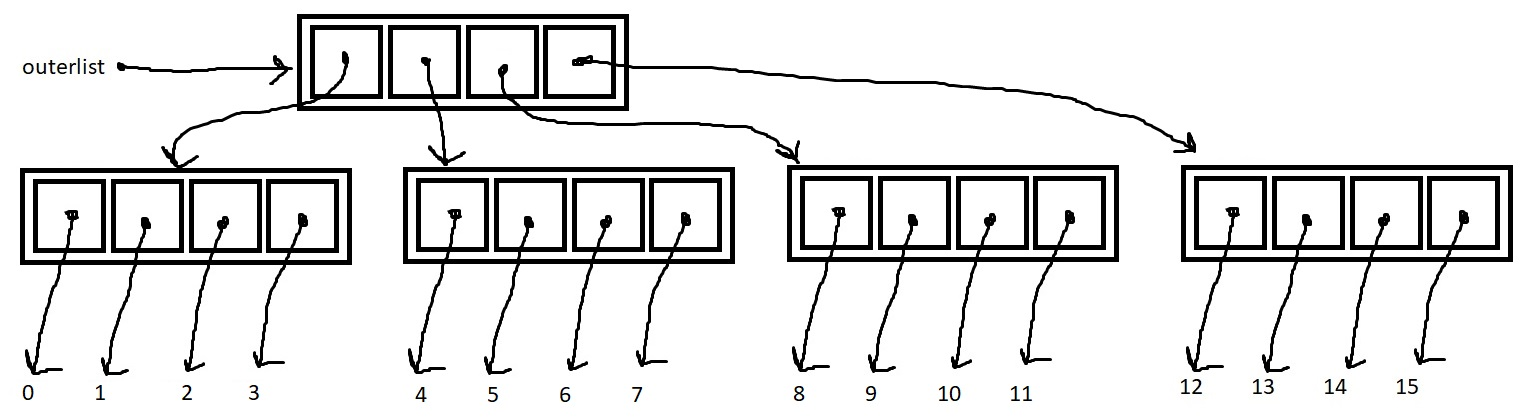
\includegraphics[width=\linewidth]{typical_student_expectation_before_activity.jpg}
\vspace{1em}
However, what we would find is that each element of the outlist just refers to the same innerList.\\
Following the links you would see all we are doing is overwriting the same list contents again and again, changing innerList from [0,0,0,0] to [0,1,2,3] to [4,5,6,7] to [8,9,10,11] to [12,13,14,15].\\

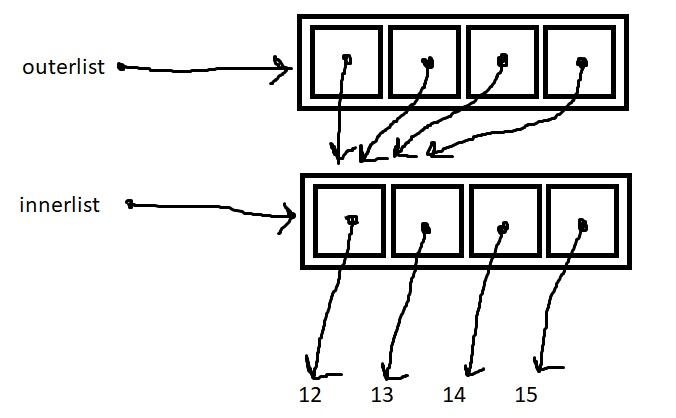
\includegraphics{solution-image.jpg}\vspace{1em}\\
To implement this algorithm so that it matches expectations of a list of lists of 0 to 15, we need \textbf{different} inner lists, one for each cell.
}

\end{document}
